\section{Introduction}
Text-to-SQL systems let users query relational databases through natural language. Recent methods improve SQL generation through prompting, specialized models and feedback \citep{gao2024dailsql,li2024codes,fan2025cyclesql}. Their evaluation relies on workloads such as Spider and BIRD \citep{yu2018spider,li2023bird}, whose questions refer to particular tables, relationships and values. Choosing a model for another database requires tasks grounded in that database. Reusing source query structures can reduce construction effort, but the resulting workload must also be assessed as a measurement instrument.

Existing approaches address different parts of this problem. RingSQL uses schema-independent templates to produce training pairs, while OmniSQL synthesizes diverse databases, queries and questions for training \citep{sterbentz2026ringsql,li2025omnisql}. SQLMorph expands joins and perturbs questions to diagnose model weaknesses \citep{malekpour2026sqlmorph}. These methods establish useful construction and diagnostic techniques. Their generation quality, structural coverage or downstream training gains do not, however, determine whether a migrated workload preserves source model comparisons or supports model selection on the target database. We study this distinction in \emph{cross-domain benchmark migration}.

\textbf{Challenges.} \emph{First, executable SQL does not establish task meaning.} Execution-based evaluation can miss semantic differences \citep{zhong2020testsuite}, and data-grounded explanations show why database contents matter when checking SQL \citep{fan2025cyclesql}. When transferring a query pattern, matching column types alone can change the entities, relationships or measures being queried. Value-linking studies further show that syntactically valid queries can use the wrong database values \citep{koukouvinis2026value}. Benchmark construction therefore needs to ground both SQL and its question in the target schema and data.

\begin{figure*}[t]
\centering
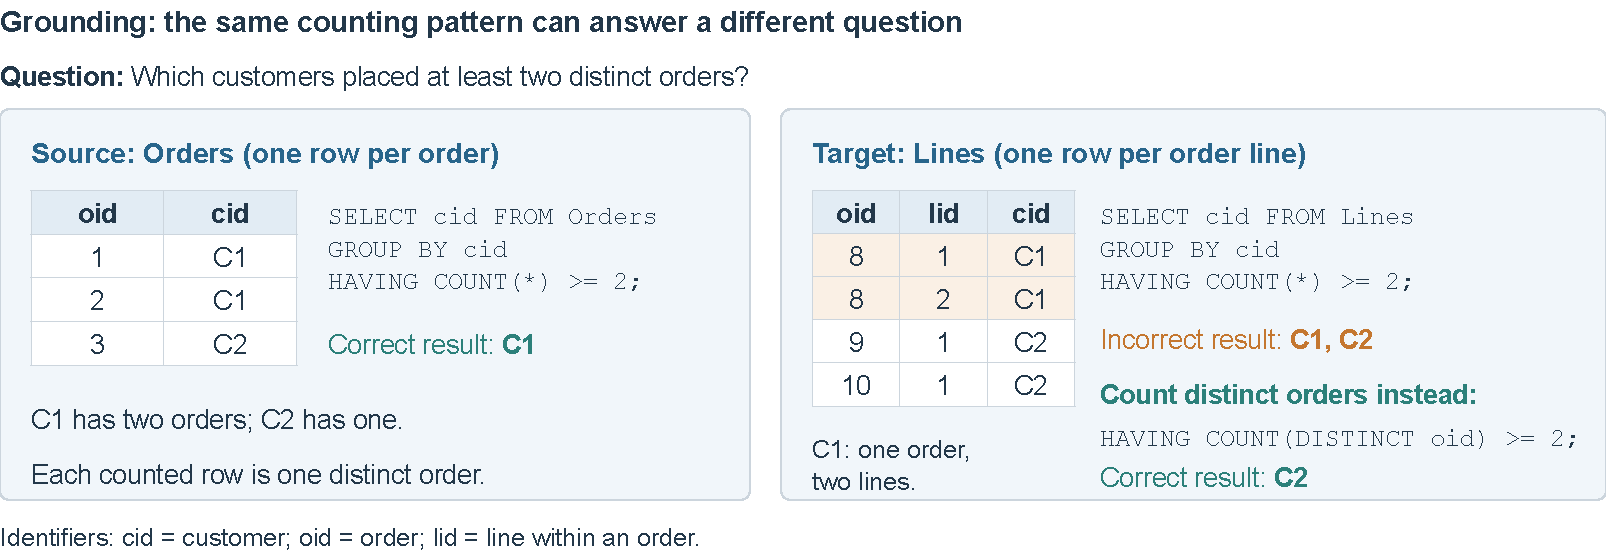
\includegraphics[width=\textwidth]{figures/current/Fig1.pdf}
\caption{An illustrative grounding error: transferring \texttt{COUNT(*)} from orders to order lines changes what is counted. Both target queries execute, but only distinct-order counting answers the question. Data are constructed for explanation.}
\label{fig:problem}
\end{figure*}

\textbf{An illustrative example.} Figure~\ref{fig:problem} asks which customers placed at least two orders. \texttt{COUNT(*) >= 2} works on source order rows. On target order lines, C1 has two rows for one order; C2 has two orders. The transferred query returns both; \texttt{COUNT(DISTINCT oid)} correctly retains C2. Execution alone cannot distinguish counting units.

\emph{Second, a valid workload can change model comparisons.} Diagnostic perturbations expose sensitivity to query structure and wording \citep{malekpour2026sqlmorph,chang2023drspider}; benchmark-design and concurrence studies also distinguish evaluation claims from the evidence needed to support them \citep{liu2024ecbd,sun2023concurrence}. Matching structural frequencies alone need not preserve model behavior. Selection can adjust frequencies only within the available candidate pool, and source fidelity need not imply agreement with target references.

Suppose models A and B score 75\% and 50\% on the source, but 50\% and 75\% on target references. Preserving source behavior favors A; target alignment favors B. Compact evaluation methods estimate performance on an existing benchmark \citep{maiapolo2024tiny}; migration changes both the database and task population.

\textbf{Our methodology.} Schema2Bench (S2B) has three modules (Fig.~\ref{fig:framework}). \emph{Benchmark Construction} instantiates source query patterns with target schemas and sampled values, then generates questions from SQL. \emph{Workload Selection} adjusts composition under fixed quotas, tightly bounds fidelity changes and identifies coverage deficits that selection cannot remove. \emph{Benchmark Evaluation} separates source fidelity from target alignment and retains unknowns in direct comparisons. Screening uses earlier outputs; selection reads no evaluator responses. Execution and consistency checks screen operational failures without certifying semantics.

\textbf{Experimental evaluation.} On eight BIRD databases with ten models, S2B improves both source fidelity and target gap over Template. It also improves Verified source fidelity over three generation-based adaptations, which attain lower target gaps. Ablations locate most improvement before selection and show how wording changes this tradeoff.

\textbf{Contributions.} We make three contributions:
\begin{enumerate}
\item \textbf{Benchmark Construction.} We construct target tasks from source SQL patterns using schema and value evidence, with explicit question--SQL alignment and failure handling (Section~\ref{sec:grounded-construction}).
\item \textbf{Workload Selection.} We bound the fidelity change from quota-constrained selection and characterize structural deficits in the candidate pool (Section~\ref{sec:quota-release}).
\item \textbf{Benchmark Evaluation.} We distinguish source fidelity from target model choice and evaluate construction, selection and wording effects under execution and semantic uncertainty (Sections~\ref{sec:measurement-stage} and~\ref{sec:experiments}).
\end{enumerate}

\section{Preliminaries}\label{sec:preliminaries}
\subsection{Text-to-SQL Tasks}
A domain is a fixed database snapshot. Task $(d_i,x_i,s_i)$ pairs question $x_i$ and reference SQL $s_i$ on domain $d_i$. Migration (Fig.~\ref{fig:framework}) constructs $N$ tasks across $D$ domains, using source queries $\mathcal S$ for patterns and statistics. A separate workload $\mathcal W_s$ provides the behavioral reference for $M\ge2$ models.

\subsection{Evaluation Objectives}
Source fidelity measures continuity with source behavior; target alignment, rankings and regret assess target model comparisons and selection (Section~\ref{sec:objectives}).

\section{Schema2Bench Overview}\label{sec:framework}
In this section, we first formulate benchmark migration in Section~\ref{sec:problem-definition}, then outline Schema2Bench in Section~\ref{sec:overview-modules}. Its three modules are \emph{Benchmark Construction}, \emph{Workload Selection} and \emph{Benchmark Evaluation}. Sections~\ref{sec:grounded-construction}, \ref{sec:quota-release} and~\ref{sec:measurement-stage} describe their implementations, respectively.

\subsection{Problem Formulation}\label{sec:problem-definition}
Candidate pool $\mathcal C$ retains IDs and evidence. Membership $z\in\{0,1\}^{|\mathcal C|}$ specifies release $\mathcal W_z$, selecting item $i$ when $z_i=1$. Strata partition candidates within domains; $A_{g,i}$ indicates membership in stratum $g$, with quota $q_g$. Feasible memberships $\mathcal F$ satisfy $Az=q$ and $\mathbf1^\top z=N$, where $\mathbf1$ is the all-ones vector. Quotas fix domain sizes $N_d>0$ and require sufficient candidates per stratum.

Given initial release $z^0\in\mathcal F$, selection seeks
\begin{equation}
 \min_{z\in\mathcal F}L_{\rm struct}(z)
 \quad\text{subject to }H(z,z^0)\le\tau.
 \label{eq:migration-selection}
\end{equation}
$L_{\rm struct}$ measures source-structure mismatch. $H$ bounds changes in source fidelity error (TEF), with tolerance $\tau$ (Section~\ref{sec:quota-release}), not absolute loss.
\subsection{Framework Overview}\label{sec:overview-modules}
Figure~\ref{fig:framework} connects candidate construction, workload selection and model evaluation on source, selected and reference tasks.

\begin{figure*}[t]
\centering
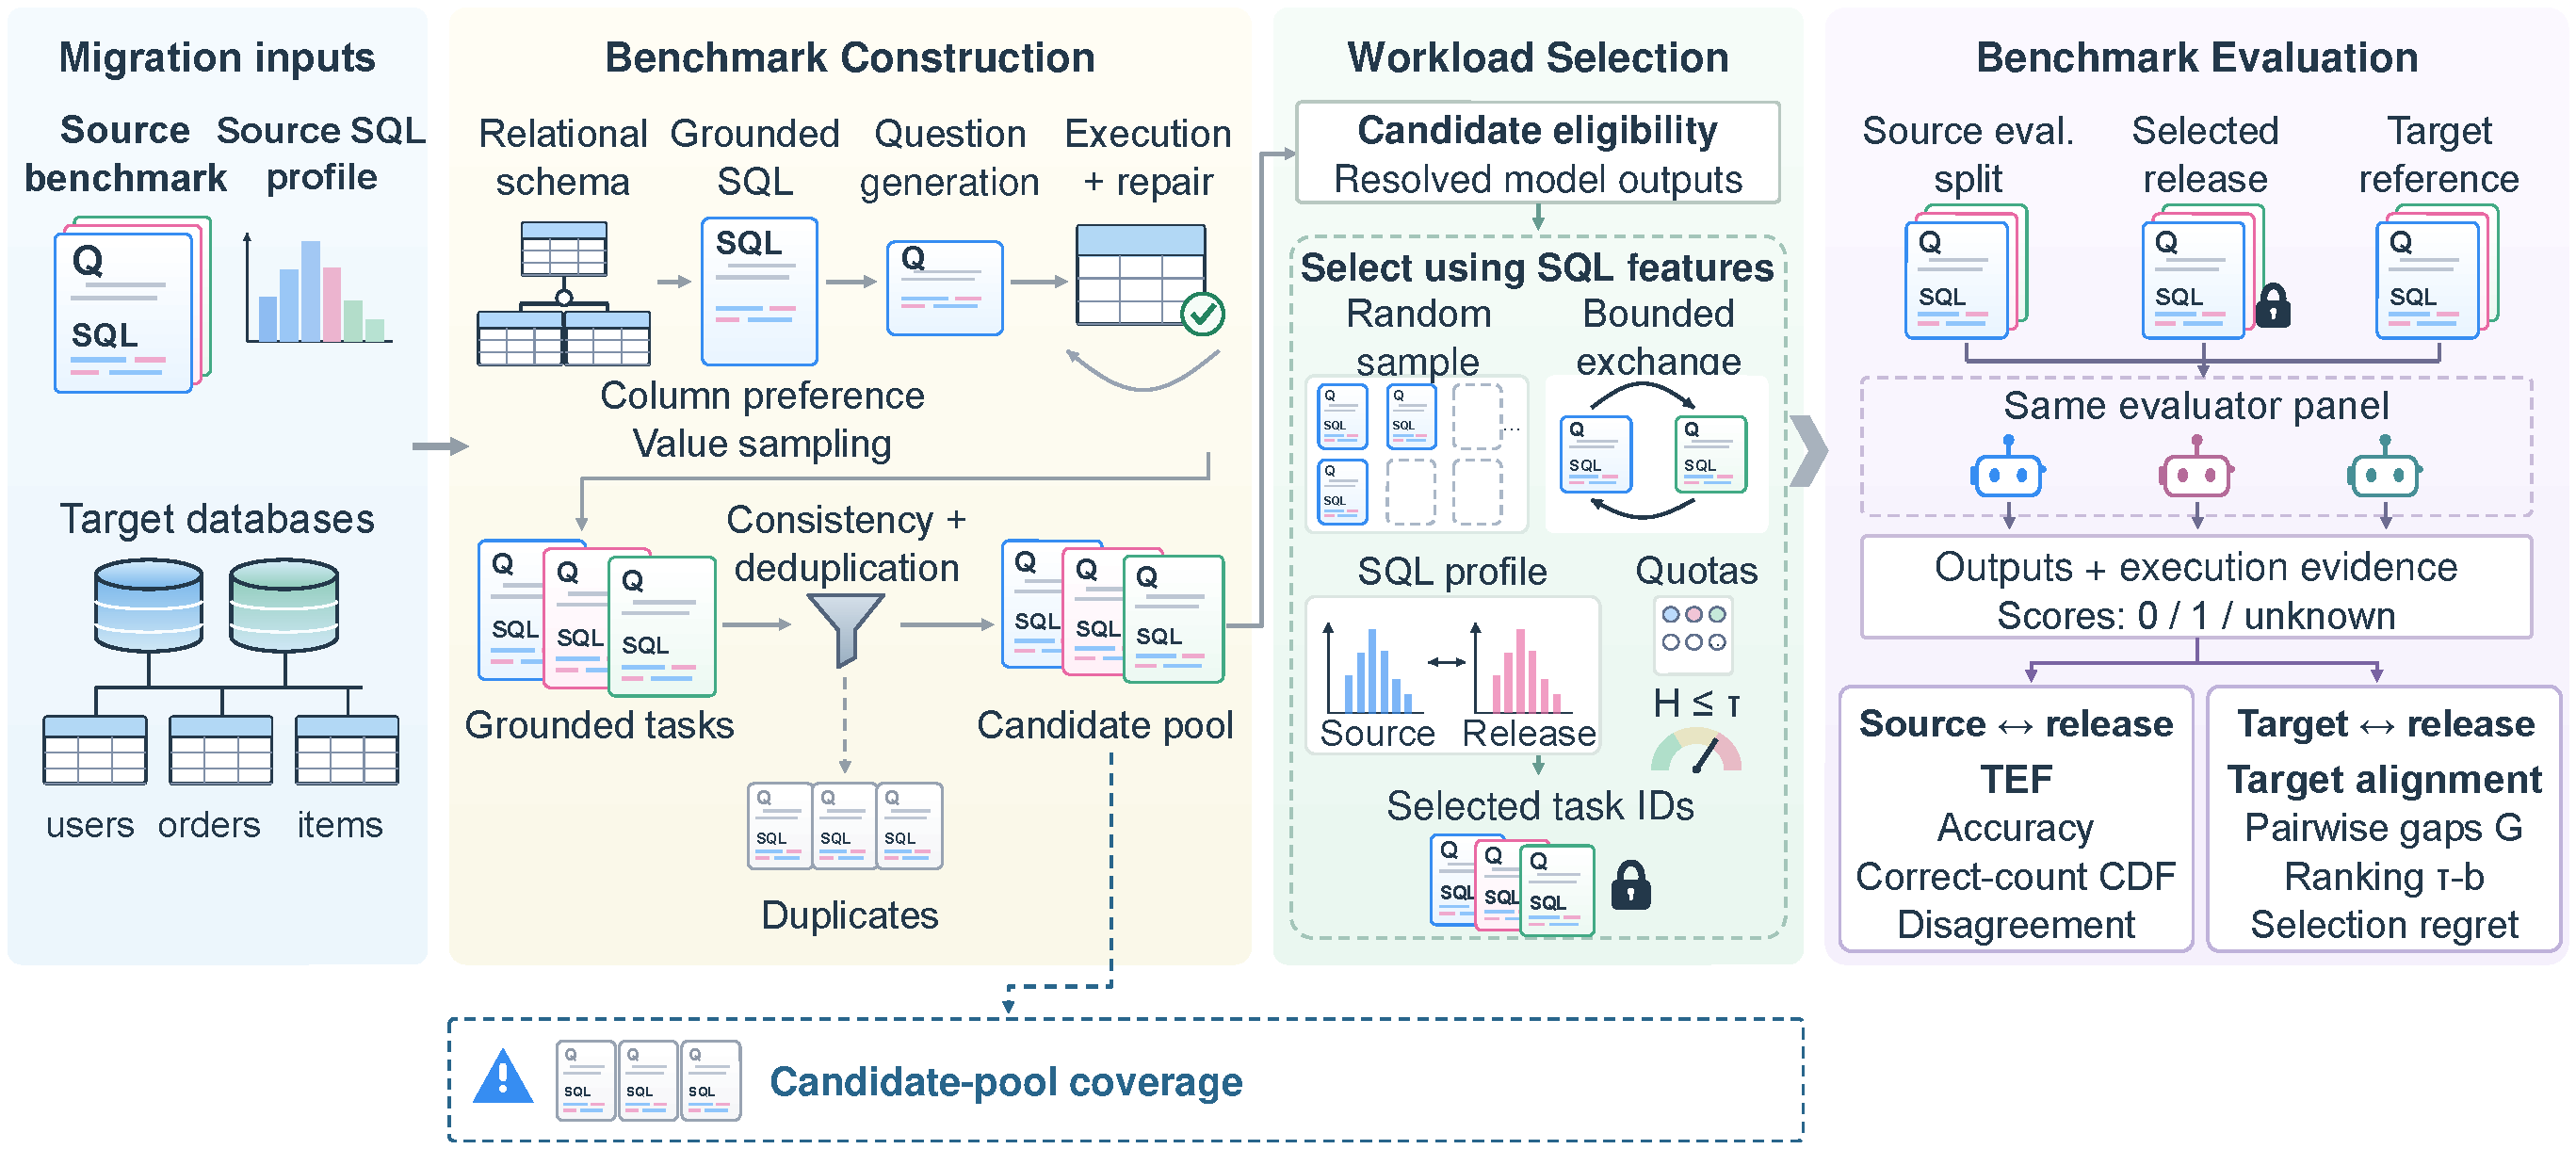
\includegraphics[width=\textwidth]{figures/current/Fig2.pdf}
\caption{The three Schema2Bench modules: Benchmark Construction, Workload Selection and Benchmark Evaluation. Q: question; CDF: cumulative distribution function; $H$: fidelity-change bound; $\tau$: tolerance; $G$: target gap; $\tau$-b: Kendall rank correlation.}
\label{fig:framework}
\end{figure*}

\section{Methodologies}\label{sec:methodology}
We detail the three modules below.

\subsection{Benchmark Construction}\label{sec:grounded-construction}

Schema2Bench instantiates source operator patterns with target tables, types, keys and sampled values, then derives questions from SQL. The evaluated implementation is programmatic; Section~\ref{sec:realization} tests LLM question generation.

\textbf{Binding operators to the database.} Columns whose names suggest identifiers are excluded from measures and descriptive projections. Text and descriptive-name cues guide projections; categorical cues guide grouping. SUM requires cues that the column represents an additive measure. Join candidates follow declared keys or entity-key heuristics. Equality predicates use observed values, with up to fifty samples per column. If a join cannot be built, the generator falls back to a grounded filter or scalar aggregate. Structural features are recomputed from the final SQL; the recorded construction stratum is retained separately.

\textbf{Keeping the question aligned with SQL.} Questions name columns, filters, join relationships and aggregation roles. For recognized joins, \texttt{COUNT(*)} describes matched rows: order-line rows in Fig.~\ref{fig:problem}. S2B does not infer a general entity-preserving \texttt{COUNT(DISTINCT)} repair; distinct-order counting requires different SQL. Relationship clarification also applies to Template.

\textbf{Admission and failure handling.} Execution checks and bounded repair handle operational failures. A final LIMIT clause requires recoverable ordering over projected columns or proof of a unique cutoff; the question must state the ordering and limit. Consistency checks screen literal, entity and ordering mismatches; deduplication removes repeated tasks. These checks reduce identifiable failure modes without certifying question--SQL meaning. Canonical IDs pair Template and S2B tasks without assuming identical semantics (Section~\ref{sec:semantic}).


\subsection{Workload Selection}\label{sec:quota-release}

\textbf{Candidate eligibility.} Definite execution scores and normal termination determine $\mathcal C$ (Section~\ref{sec:design}). This screen depends on outputs; selection reads only SQL features, schema evidence, metadata and a seed. Main-study strata combine domain and recorded construction group.

\textbf{Selection using SQL features.} Sampling $q_g$ candidates per stratum gives initial release $z^0$. Exchanges improve structural matching while limiting their possible effect on the measured response profile. They target Eq.~\eqref{eq:migration-selection} while preserving quotas. Structural loss averages operator-event and SQL-only difficulty total variation (TV), six shape deviations, relative mean join-count and SQL-length errors:
\begin{align}
 L_{\rm struct}(z)=\frac15\bigg(&\frac{\|\widehat P_o-P_o^*\|_1}{2}
 +\frac{\|\widehat P_d-P_d^*\|_1}{2}
 +\frac{\|\widehat P_h-P_h^*\|_1}{6}\nonumber\\
 &+\frac{|\widehat j-j^*|}{j^*}
 +\frac{|\widehat\ell-\ell^*|}{\ell^*}\bigg).
 \label{eq:struct-expanded}
\end{align}
$P_o,P_d$ describe operator-event and difficulty distributions; $P_h$ contains rates of filtering, joins, grouping, aggregation, ordering and LIMIT. $j,\ell$ denote mean joins and SQL length in whitespace-separated tokens. Hats and stars denote release and source statistics, respectively; $\|\cdot\|_1$ sums absolute coordinates. Difficulty and shapes count tasks. Positive source means allow relative errors above one.

SQL-only difficulty sums joins, twice the additional SELECT and set-operator counts (UNION, INTERSECT, EXCEPT), and indicators for grouping, HAVING, aggregation, ordering, CASE, DISTINCT and at least two AND or OR tokens. Scores $\le1$, 2--3 and $\ge4$ define easy, medium and hard, differing from Spider labels and behavioral or semantic difficulty.

Let $r_d$ count tasks removed from initial release $z^0$ in domain $d$. The budget function $H=H(z,z^0)$ is
\begin{equation}
 H=\sum_d(w_d^A+w_d^R)\frac{r_d}{N_d}
 =\frac rN+\frac1D\sum_d\frac{r_d}{N_d},\qquad r=\sum_dr_d,
 \label{eq:budget}
\end{equation}
where $w_d^A=1/D$ weights accuracy and $w_d^R=N_d/N$ weights the correct-count cumulative distribution function (CDF) and disagreement across domains (Section~\ref{sec:objectives}). Each exchange $e$ replaces an initial item with an unused candidate outside the initial release in the same stratum. For resulting membership $z'$, gain is $\Delta_e=L_{\rm struct}(z)-L_{\rm struct}(z')$ and cost is $c_d=1/N+1/(DN_d)$. Choose the largest positive $\Delta_e/c_d$ fitting the budget, breaking ties by resulting loss and IDs. Update $z,H$; stop at no admissible improvement or the step cap. Feasibility and decreasing structural loss hold, without global optimality.

For fixed source moments, joint response laws and domain counts, $|L_{\tef}(z)-L_{\tef}(z^0)|\le H$. Response vectors at Hamming distance $h_H$ change accuracy by at most $h_H/M$, and CDF plus half-weighted disagreement by at most $\frac{h_H}M+\frac{h_H(M-h_H)}{M(M-1)}\le1$. Coupling removed and added items gives Eq.~\eqref{eq:budget}, attained by all-zero source and initial responses with all-one replacements. This perturbation bound also holds in expectation under fixed joint laws, including deterministic saved responses.


\subsubsection{Candidate Coverage}\label{sec:pool-diagnostic}

Over SQL types $T$, such as easy, medium and hard queries, let $p$ and $q_z$ denote source and release proportions, distinct from quotas $q$. The convex hull $\mathcal Q=\operatorname{conv}\{q_z:z\in\mathcal F\}$ contains their feasible mixtures $v$. With dual type weights $h$, the minimum type mismatch is
\begin{equation}
\delta_{\rm sup}=\min_{v\in\mathcal Q}\operatorname{TV}(p,v)
=\max_{h\in[0,1]^{|T|}}\left(h^\top p-\max_{z\in\mathcal F}h^\top q_z\right).
\end{equation}
The coverage lower bound $\delta_{\rm sup}$ uses a bounded-count linear program (LP) relaxation and sorted dual weights. Omitting $H\le\tau$ preserves validity for budgeted selection. An attaining integer release certifies optimal type matching; otherwise integrality may leave a gap. With unchanged feasible quotas, adding $b$ eligible candidates reduces TV over pooled tasks by at most $b/N$: replace new selections with unused old items in the same strata. This bounds structural capacity, not TEF (Section~\ref{sec:current-support}); Section~\ref{sec:acquisition} tests acquisition.


\subsection{Benchmark Evaluation}\label{sec:measurement-stage}
The same $M$ models answer source, release and reference tasks; unresolved scores remain unknown.

\subsubsection{Evaluation Measures}\label{sec:objectives}

\textbf{Source fidelity (TEF).} $Y_i\in\{0,1\}^M$ contains task $i$'s execution-match indicators, with $m,n$ indexing models. TEF compares accuracy, correct-count CDF indicators $\mathbf1\{\sum_mY_{i,m}\le k\}$, $k=0,\ldots,M-1$, and disagreement $|Y_{i,m}-Y_{i,n}|$. Here $\mathbf1\{\cdot\}$ is one when true, zero otherwise. With source and release feature means $\Psi_s,\Psi_z$,
\begin{equation}
 L_{\tef}(z)=\sum_\nu w_\nu|\Psi_{z,\nu}-\Psi_{s,\nu}|
 =D_{\rm diff}+D_{\rm acc}+\tfrac12D_{\rm dis}.
 \label{eq:tef}
\end{equation}
$\nu$ indexes coordinates with weights $w_\nu$: $1/M$ for accuracy and CDF and $1/(2\binom M2)$ for disagreement. $D_{\rm diff},D_{\rm acc},D_{\rm dis}$ are mean absolute differences in CDF, accuracy and disagreement, respectively. For selected domain items $z_d=\{i:z_i=1,d_i=d\}$, accuracy coordinate $\Psi^A_{z,m}$ averages databases equally:
\begin{equation}
 \Psi^A_{z,m}=\frac1D\sum_d\frac1{N_d}\sum_{i\in z_d}Y_{i,m}.
\end{equation}
CDF and disagreement pool tasks; source accuracy averages 20 databases. Equal target quotas do not remove unequal source sizes. Block weights $(1,1,1/2)$ define the convention; Section~\ref{sec:sensitivity} varies these priorities over the nonnegative weight region without changing the structural objective.

\textbf{Target alignment.} For construction $c$, let $a^r_{d,m}$ and $a^c_{d,m}$ be model $m$'s execution-match rates on reference and constructed tasks in domain $d$. Target gap measures differences between their pairwise accuracy gaps:
\begin{equation}
 G(c)=\frac1D\sum_d\frac1{\binom M2}\sum_{m<n}
 \left|(a^r_{d,m}-a^r_{d,n})-(a^c_{d,m}-a^c_{d,n})\right|.
 \label{eq:gap}
\end{equation}
Lower TEF and gap are better. For constructions $a,b$, $\Delta G(a,b)=G(a)-G(b)$ and $\Delta\mathrm{TEF}$ use first-minus-second losses; negative favors the first. $I_G=G(\mathrm{Template})-G(\mathrm{S2B})$ reports positive improvement. Multiplying by 100 gives gap percentage points (pp), distinct from accuracy changes. Domain-mean Kendall $\tau$-b measures ranking with ties; regret is target accuracy lost by choosing a release winner. Common accuracy shifts preserve gaps, while near ties can reverse rankings.


\subsubsection{Execution Scoring}\label{sec:scoring}

Base scoring compares result values and column counts, including empty-result widths. Non-stop or unresolved outputs receive $[0,1]$; parser rejection or unordered LIMIT alone does not prove error. Neither scoring layer certifies question--SQL meaning.

The Verified layer resolves unknowns using SQLite errors, row counts, unique ordering and checks of possible LIMIT results tied to original outputs (Table~\ref{tab:main}). 
\subsubsection{Comparisons with Unknown Scores}

Unknown scores induce feature intervals. Direct contrasts share source and reference uncertainty; target outcomes remain separate unless prompts and outputs match (Section~\ref{sec:ablation}). Coordinate relaxation gives conservative outer bounds, not confidence intervals or necessarily attainable endpoints. We never subtract independently optimized row bounds.

Bootstrap intervals condition on stated populations, weights and units; shared models and pools make pairs and releases dependent.

Lower and upper score bounds $[l_{i,m},u_{i,m}]$ are $[0,0]$, $[1,1]$ or $[0,1]$ for mismatch, match or unknown. Weighted means bound accuracy; CDF contributions lie between $\mathbf1\{\sum_m u_{i,m}\le k\}$ and $\mathbf1\{\sum_m l_{i,m}\le k\}$. Disagreement is fixed when both scores are fixed, otherwise relaxed to $[0,1]$. 

For method-feature intervals $A=[a_-,a_+]$, $B=[b_-,b_+]$, the minimum and maximum absolute distances are
\begin{align}
 d_-(A,B)&=\max(a_- - b_+,b_- - a_+,0),\\
 d_+(A,B)&=\max(|a_- - b_+|,|a_+ - b_-|).
\end{align}
For shared source-feature interval $S$, the discrepancy difference (first minus second) has lower and upper bounds
\begin{align}
 \underline\Delta&=\min_{s\in S}\{d_-(\{s\},A)-d_+(\{s\},B)\},\\
 \overline\Delta&=\max_{s\in S}\{d_+(\{s\},A)-d_-(\{s\},B)\}.
 \label{eq:shared-contrast}
\end{align}
Both terms share source value $s\in S$. We sum weighted coordinate bounds, evaluating endpoints and piecewise-linear breakpoints. Gap contrasts similarly share signed target-reference model gaps.

\section{Experimental Results}\label{sec:experiments}
We compare source fidelity across methods (Section~\ref{sec:measurement}), the contributions of construction and selection (Section~\ref{sec:construction}), and robustness across assumptions and domains (Sections~\ref{sec:robustness}--\ref{sec:external}). TEF assesses source continuity; gap, ranking and regret test whether this also supports target model choice.

\subsection{Experimental Setup}\label{sec:design}
\subsubsection{Datasets and Models}

The primary comparison uses eight BIRD databases (Table~\ref{tab:screening}), ten models, 2,000 tasks per method and 906 shared references. Spider supplies 7,000 training queries for source profiles and 1,034 development tasks across 20 databases for evaluation. Prompts include data definition language (DDL) schemas from retained snapshots.

The panel comprises Qwen3-4B (Instruct-2507), Granite-3.3-8B-Instruct \citep{ibm2025granite}, Qwen2.5-Coder-7B-Instruct \citep{hui2024qwencoder}, Qwen2.5-7B-Instruct, Llama-3.1-8B-Instruct \citep{grattafiori2024llama3}, Mistral-7B-Instruct-v0.3 \citep{jiang2023mistral,mistral2024instruct03}, Qwen2.5-14B-Instruct, Qwen3-8B, Gemma-2-9B-it \citep{gemma2024gemma2} and Phi-4 \citep{abdin2024phi4}. Qwen2.5-7B also participates in generation \citep{qwen2024qwen25}.

\paragraph{Initial qualification result}
The original workload improved in five of eight domains, below the preregistered six-domain requirement. Later Qwen3-8B non-thinking evaluations \citep{yang2025qwen3} and scoring changes do not revise this failure.

\paragraph{Candidate screening and selection}
Both tasks in each pair require normal output termination and definite ten-model scores, using compilation and row-count evidence. Incorrect responses qualify; unresolved or truncated responses do not. Most exclusions involve timeouts or unprojected ordering columns (Table~\ref{tab:screening}). Reasons can overlap and exclude earlier generation failures.

We sample 250 pairs per domain within strata from the 3,778-pair pool using proportional largest-remainder quotas. S2B features determine both arms' membership before cached scores are read; Template is not independently optimized. Equal quotas and $H\le0.01$ allow ten equal-cost swaps, preventing isolation of normalization benefits. Ten releases overlap; scoring layers share tasks. Outcome-dependent eligibility and unequal precision remain limitations.

\begin{table}[t]\centering\small
\caption{Available $\to$ retained candidates and references after ten-model eligibility screening. Each release selects 250 pairs per domain.}
\label{tab:screening}
\begin{tabular}{lrr}\toprule
Domain & Candidate pairs & Reference items\\\midrule
California schools &703$\to$703&85$\to$55\\
Card games &460$\to$453&171$\to$154\\
Codebase community &373$\to$356&176$\to$153\\
European football &613$\to$601&123$\to$91\\
Financial &383$\to$382&101$\to$82\\
Formula 1 &484$\to$478&172$\to$127\\
Superhero &508$\to$501&129$\to$118\\
Thrombosis prediction &311$\to$304&161$\to$126\\\midrule
Total &3,835$\to$3,778&1,118$\to$906\\\bottomrule
\end{tabular}\end{table}


\subsubsection{Baselines}\label{sec:comparators}

Template tests structural reuse without S2B's grounding; both share the paired pool (Section~\ref{sec:framework}). Three external adaptations test generation workflows as benchmark constructors. Ring combines template SQL with Qwen-generated questions. Omni reuses SQL and question generation components with local Qwen models. Synth uses the author's synthesis, question generation, backtranslation and self-comparison workflow with local Qwen, removing its 25-row cap.\footnote{SynthSQL toolkit: \url{https://github.com/NeginKhalifat/SQL-benchmark}, retained commit \texttt{dff8c75e}. It is distinct from SING-SQL and SynSQL.} These adaptations do not reproduce the complete original systems. Evaluation sizes are fixed; generation budgets differ (Table~\ref{tab:cost}).

Each external method supplies one unpaired set of 2,000 tasks. Omni replaces duplicates before response inspection; Synth expands adaptively and deduplicates in fixed order. Synth combines reused and new outputs with different batch and key-value cache settings; interrupted shards leave 366 tasks without post-run model checks.


\subsubsection{Scoring Settings}
Both scoring layers use the same tasks. Verified scoring resolves unknowns using saved execution evidence, with unequal coverage concentrated in California for the first four methods. Detailed score counts accompany the artifacts; semantic assessment is separate (Section~\ref{sec:semantic}).


\subsection{Main Results}\label{sec:measurement}

\begin{table*}[t]
\centering\small
\setlength{\tabcolsep}{5pt}
\caption{First release: 2,000 tasks per method, ten models, 906 target references and 1,034 Spider items. Lower is better. Direct TEF differences share source unknowns; negative favors S2B. Unknowns count scores out of 20,000. Bold marks established improvements, comparing S2B with Template for absolute scores and with each stated comparator for differences.}
\label{tab:main}
\begin{tabular}{lrrrr}\toprule
Method & Target gap $G\downarrow$ & Spider--BIRD TEF $\downarrow$ & Direct $\Delta\mathrm{TEF}$ & Unknown\\\midrule
\multicolumn{5}{l}{\textit{Verified execution scoring}}\\
Template & $[0.224967, 0.224967]$ & $[0.243915, 0.390986]$ & $\boldsymbol{[-0.131730, -0.079099]}$ & 0\\
S2B & $\boldsymbol{[0.169275, 0.169275]}$ & $\boldsymbol{[0.138501, 0.283651]}$ & $0$ & 0\\
RingSQL-style adaptation & $[0.096309, 0.100791]$ & $[0.283403, 0.435663]$ & $\boldsymbol{[-0.233594, -0.061506]}$ & 46\\
OmniSQL component adaptation & $[0.029731, 0.134760]$ & $[0.564696, 0.862439]$ & $\boldsymbol{[-0.665769, -0.324655]}$ & 1,290\\
SynthSQL-style local adaptation & $[0.013004, 0.166928]$ & $[0.268596, 0.642072]$ & $\boldsymbol{[-0.453605, -0.021084]}$ & 2,040\\
\midrule
\multicolumn{5}{l}{\textit{Base layer: strict execution and output-shape checks}}\\
Template & $[0.178882, 0.262025]$ & $[0.205735, 0.426469]$ & $[-0.193294, +0.005344]$ & 430\\
S2B & $[0.117662, 0.208049]$ & $[0.111299, 0.334757]$ & $0$ & 537\\
RingSQL-style adaptation & $[0.059199, 0.138379]$ & $[0.241426, 0.462380]$ & $[-0.293401, +0.034557]$ & 445\\
OmniSQL component adaptation & $[0.010465, 0.190895]$ & $[0.488896, 0.898945]$ & $\boldsymbol{[-0.734008, -0.195186]}$ & 2,066\\
SynthSQL-style local adaptation & $[0.000000, 0.345368]$ & $[0.103282, 0.861883]$ & $[-0.686921, +0.198272]$ & 5,149\\
\bottomrule
\end{tabular}
\end{table*}
\begin{figure*}[t]
\centering
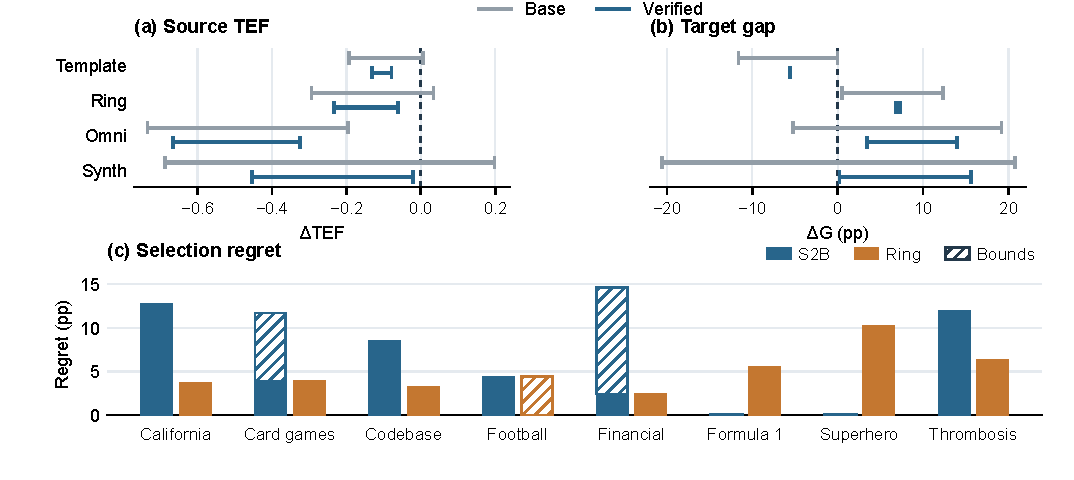
\includegraphics[width=\textwidth]{figures/current/Fig3.pdf}
\caption{First-release source TEF, target gap and model-selection regret. Panels (a--b) compare S2B with each method; panel (c) compares S2B and Ring by domain. Caps indicate bounds; ticks indicate coincident endpoints.}
\label{fig:main-contrasts}
\end{figure*}

\subsubsection{Source Fidelity and Target Alignment}
Schema2Bench improves both objectives over Template: lower source TEF and a \textbf{0.055693} reduction in Verified target gap (Table~\ref{tab:main}). All four direct TEF bounds are strictly negative, establishing a fidelity advantage over the three generation-based adaptations despite overlapping marginal intervals. Ring, Omni and Synth attain lower gaps. S2B therefore offers better source continuity, while target alignment favors those alternatives.

All four mean Verified TEF contrasts remain negative across ten overlapping releases using fixed external sets, testing membership sensitivity rather than independent construction. Base mean bounds cross zero for Template, Ring and Synth; only the Omni contrast remains negative. The advantage over all four methods depends on additional execution evidence.

\subsubsection{Model Ranking}
Average model ordering also improves over Template: across ten Verified releases, mean gap falls from 0.224640 to 0.168988 (\textbf{5.5652 pp}) and mean domain $\tau$-b rises from 0.2292 to 0.3272. California and codebase lose rank agreement, limiting the domain-level conclusion.

For each seed, 1,000 bootstrap draws separately resample matched SQL-skeleton clusters and references. All ten rank-difference estimates are positive; eight conditional 95\% intervals exclude zero. These intervals omit missingness and pool selection.

\subsubsection{Model Selection}\label{sec:decision}
We test whether fidelity improves model selection using a regret rule fixed before this post-hoc calculation. It retains all possible winners under ties and unknowns, without ranking midpoints.
\begin{table*}[t]\centering\small
\caption{Model-selection regret in accuracy percentage points, including all possible tied winners. Mean and worst denote domain average and maximum; 906 and 1,118 are reference counts. Bounds are conservative; overall first and second ranks remain unresolved.}
\label{tab:regret}
\begin{tabular}{lrrrrr}\toprule
Method & 906: base mean & 906: verified mean & 906: verified worst & 1,118: base mean & 1,118: verified mean\\\midrule
Template & $[6.138, 8.979]$ & $[6.718, 7.854]$ & $[10.317, 12.727]$ & $[0.556, 19.177]$ & $[2.213, 14.329]$\\
S2B & $[4.122, 9.106]$ & $[5.482, 7.981]$ & $[12.727, 14.634]$ & $[0.071, 19.192]$ & $[2.500, 14.417]$\\
Ring & $[2.887, 8.100]$ & $[4.409, 4.958]$ & $10.169$ & $[0.484, 18.847]$ & $[1.547, 11.519]$\\
Omni & $[0.000, 17.895]$ & $[0.794, 12.246]$ & $[6.349, 19.512]$ & $[0.000, 28.023]$ & $[0.000, 17.857]$\\
Synth & $[0.000, 27.258]$ & $[0.000, 19.046]$ & $[0.000, 25.490]$ & $[0.000, 37.369]$ & $[0.000, 23.858]$\\
\bottomrule\end{tabular}\end{table*}

With 906 references and Verified scoring, mean regret favors Ring despite S2B's lower TEF (Table~\ref{tab:regret}). Domain comparisons favor Ring in California and codebase, and S2B in Formula 1 and superhero. Omni and Synth bounds remain wide. Figure~\ref{fig:main-contrasts}(c) distinguishes lower bounds from remaining ranges.

All 1,118 references yield overlapping S2B and Ring bounds, with 1,356 Base and 706 Verified unknowns. Ten-release regret ranges are retained with the artifacts.

\subsection{Ablation Studies}\label{sec:construction}

We test grounding choices and question wording before examining selection (Fig.~\ref{fig:construction-effects}). Grounding controls use separate paired releases; rewriting fixes SQL; selection controls share the pool. Their effects do not additively decompose the main improvement.

\begin{figure*}[t]
\centering
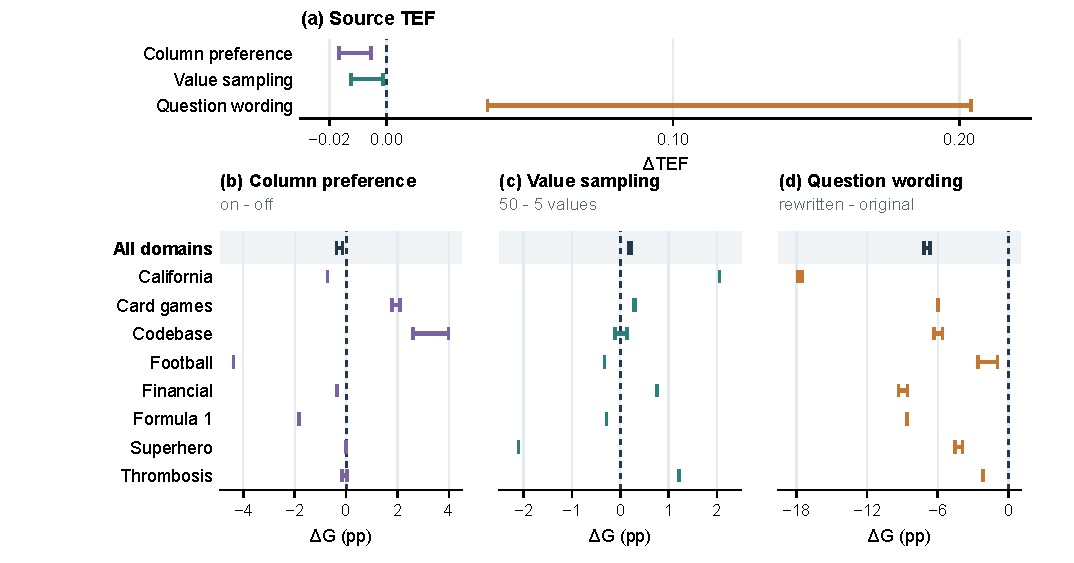
\includegraphics[width=\textwidth]{figures/current/Fig4.pdf}
\caption{Construction controls under Verified scoring: source TEF and target-gap differences across domains.}
\label{fig:construction-effects}
\end{figure*}

\begin{table}[t]\centering\small
\caption{Selection over ten overlapping 2,000-task releases. (a) BIRD, ten models: positive $I_G$ favors S2B over Template. (b) Earlier seven-database, seven-model study: lower is better. Best and second values are marked separately within each panel and metric.}
\label{tab:anchor}
\begin{tabular}{lrrr}\toprule
\multicolumn{4}{l}{\textit{(a) BIRD: construction versus selection}}\\
Selection & Swaps & $H$ & $I_G\uparrow$ (pp)\\\midrule
Initial stratified sample &0&0&5.5386\\
Matched random swaps &10&0.01&\underline{5.5449}\\
Structural adjustment &10&0.01&\textbf{5.5652}\\\midrule
\multicolumn{4}{l}{\textit{(b) Seven additional databases: selection}}\\
Selector & \multicolumn{2}{c}{Structural loss} & TEF\\\midrule
Stratified random & \multicolumn{2}{c}{0.269519} &0.050071\\
Structural greedy & \multicolumn{2}{c}{\textbf{0.213055}} &\underline{0.048692}\\
Bounded selection & \multicolumn{2}{c}{\underline{0.260790}} &\textbf{0.047229}\\\bottomrule
\end{tabular}\end{table}

\subsubsection{Column Preference and Value Sampling}\label{sec:ablation}
Separate paired releases disable descriptive-column preference or reduce sampling from fifty values to five. They use the main models, source tasks and references, with 38 strata, 250 tasks per domain in each arm and $H=0.01$. Attempts share random states and plans; separately deduplicated candidates must qualify in the same final stratum.

The preference control retains identifier filtering, text preference, grounding and admission rules. Programmatic question generation uses eight-second and 1,000-row limits. Four domains require 1,600 extra slots each before freezing; the arms share 1,159 of 2,000 question--SQL pairs. Sampling uses 2,400 slots per domain in each arm: fifty and five values admit 7,131 and 6,149 candidates, respectively, with 5,375 joint admissions and 769 shared release slots. Astra supports both versions of 80 sampling-control pairs, 24 with identical prompts, using exposed controls. Admission differences remain part of the comparison.

SQLite compilation resolves 827 preference and 903 sampling-control parser rejections as mismatches without rewriting SQL. Identical requests and outputs share unknowns across arms; others remain relaxed. This post-hoc treatment preserves scores, membership and identity records. Table~\ref{tab:ablation-layers} also retains earlier independent-arm bounds.

\begin{table*}[t]\centering\small
\caption{Separate construction controls under Verified scoring. Negative favors full preference or fifty values. Bounds with shared variables bind identical outcomes; independent-arm bounds retain the earlier relaxation.}
\label{tab:ablation-layers}
\begin{tabular}{llrr}\toprule
Intervention & Unknown-variable treatment & Direct TEF difference & Direct target-gap difference\\\midrule
Column preference & Independent arms & $[-0.029752,+0.008062]$ & $[-0.011942,+0.006559]$\\
Column preference & Shared identical requests & $\boldsymbol{[-0.016593,-0.005466]}$ & $\boldsymbol{[-0.003816,-0.001425]}$\\
50 versus 5 values & Independent arms & $[-0.024987,+0.011333]$ & $[-0.006878,+0.011031]$\\
50 versus 5 values & Shared identical requests & $\boldsymbol{[-0.012477,-0.001261]}$ & $[+0.001863,+0.002221]$\\\bottomrule
\end{tabular}\end{table*}

With shared unknowns, column preference improves both metrics; deeper sampling improves TEF at a small gap cost (Table~\ref{tab:ablation-layers}). Base TEF favors both, with unresolved gaps. LP checks reproduce 26 aggregate and domain contrasts per intervention.

Column preference increases the gap in card games and codebase (Fig.~\ref{fig:construction-effects}(b)). Excluding European football changes its seven-domain mean difference to $[+0.001899,+0.004625]$; excluding Formula 1 leaves it unresolved. Sampling effects also vary by domain.

\paragraph{Value sampling on additional databases}
Four SynSQL-2.5M training databases \citep{li2025omnisql} supply 1,000 identical pairs; BIRD \texttt{student\_club} changes 150 of 250 pairs. Three further targets miss quotas. Across thirteen domains, 3,250 tasks per arm and 1,733 references give Verified TEF and gap differences of $[-0.050927,+0.049902]$ and $[-0.029026,+0.030559]$, respectively. Adding SQLite evidence only on the original eight domains gives $[-0.013017,+0.011489]$ and $[-0.004886,+0.007287]$. Both remain unresolved. Unchanged pairs, unequal evidence and synthetic training-data overlap limit independent replication.

\subsubsection{Question Generation}\label{sec:realization}
We isolate wording effects by holding SQL fixed. A preliminary comparison identifies 1,973 Ring--Template pairs sharing SQL, domains and schema prefixes but differing in questions. Their Ring-minus-Template execution-match difference is $[-13.96,-13.73]$ pp, motivating this intervention.

We retain all 2,000 first-release S2B queries and quotas, using Ring-style Qwen2.5-7B question generation. The plan and 160-item audit, with 20 items per domain, precede generation. This yields 1,999 correctly formatted questions and 19,990 predictions; the remaining item stays unknown.

Rewriting reduces Verified gap in all eight domains and aggregate Base gap, but increases Verified TEF (Table~\ref{tab:realization-results}). Concordant model pairs increase; regret intervals overlap. Against Ring, TEF is lower but the gap difference remains unresolved.

\begin{table*}[t]\centering\small
\caption{Question rewriting with fixed SQL on the first release. Panel (a) reports Verified results; concordances count definite agreement in ordering among 360 dependent model pairs. Regret is in accuracy percentage points. Bold in (a) compares rewriting with the original; (b) reports direct difference bounds, where negative favors rewriting.}
\label{tab:realization-results}
\begin{tabular}{lrrr}\toprule
\multicolumn{4}{l}{\textit{(a) Overall results}}\\
Release & Target gap $\downarrow$ & Definite concordances $\uparrow$ & Mean regret (pp) $\downarrow$\\\midrule
Original S2B & $0.169275$ & 229/360 & $[5.48,7.98]$\\
Rewritten S2B & $\boldsymbol{[0.097452,0.102706]}$ & \textbf{248/360} & $[4.30,5.57]$\\
Ring & $[0.096309,0.100791]$ & 246/360 & $[4.41,4.96]$\\\midrule
\multicolumn{4}{l}{\textit{(b) Direct differences}}\\
Contrast & Scoring & $\Delta\mathrm{TEF}$ & $\Delta G$\\\midrule
Rewritten $-$ original S2B & Verified & $[+0.035191,+0.203968]$ & $\boldsymbol{[-0.071823,-0.066569]}$\\
Rewritten $-$ Ring & Verified & $\boldsymbol{[-0.046174,-0.009796]}$ & $[-0.003339,+0.006397]$\\
Rewritten $-$ original S2B & Base & Crosses zero & $\boldsymbol{[-0.120114,-0.002971]}$\\\bottomrule
\end{tabular}\end{table*}

Using exposed synthetic controls, Terra supports 117 of 160 tasks. Changes in task meaning remain a concern despite fixed SQL (Section~\ref{sec:risk-sources}).



\begin{table*}[t]\centering\small
\caption{Recorded tokens including failures. Evaluation rows are release means; generation scopes differ. Unequal scopes are unranked.}
\label{tab:cost}
\begin{tabular}{lrrl}\toprule
Stage & Input tokens & Output tokens & Scope\\\midrule
Template evaluation &22,906,504&1,170,824&20,000 model--item records per release\\
S2B evaluation &22,936,877&1,143,564&20,000 model--item records per release\\
Spider summary evaluation &1,816,236&370,097&10,340 source records\\
Spider DDL evaluation &4,221,154&370,682&10,340 source records\\
Synth final evaluation &22,041,137&804,975&20,000 records; 5,080 reused\\\midrule
Ring question generation &417,101&125,758&2,400 records; excludes template SQL\\
Omni SQL and question generation &31,498,785&5,905,818&Initial, additional and reserve generation\\
Synth all recorded generation &553,507,001&15,411,464&258,674 calls, including failed or stopped attempts\\\bottomrule
\end{tabular}\end{table*}

\subsubsection{Workload Selection}\label{sec:selection}
Most gap improvement over Template precedes selection (Table~\ref{tab:anchor}(a)). Structural adjustment adds only 0.0204 pp over matched random swaps under Verified scoring, improving nine of ten seeds. The 16 alternatives per seed match screening, directed removals, swaps and $H$. Selection controls composition within the fidelity bound, with little additional gap benefit.



Template and S2B have initial mean $\tau$-b values of 0.2312 and 0.3270, versus 0.2292 and 0.3272 after adjustment. Relative to matched random swaps, TEF changes by $[+0.000227,+0.000977]$ with source summaries (eight seeds unfavorable; two unresolved) and $[-0.000777,+0.000452]$ with source DDL (two favorable; eight unresolved).

\paragraph{Seven additional databases}
Earlier seven-model results favor bounded selection for TEF and greedy selection for structural loss; all 14 swaps occur in TPC-DS (Table~\ref{tab:anchor}(b)). Repair improves yield, but controlled construction produces fewer tasks at higher cost than Ring, without establishing main-study component benefits.

\subsubsection{Candidate Coverage}\label{sec:current-support}

Coverage analysis identifies when further selection cannot improve the workload. The pool has 311 easy, 2,688 medium and 779 hard tasks, versus source proportions $(0.464,0.348,0.188)$. The 38 quotas allow at most 173 easy items per 2,000; $h=(1,0,0)$ certifies $0.464-173/2000=0.3775$. Both $(173,1302,525)$ and the current $(173,1376,451)$ attain it. The latter meets $H=0.01$, certifying that selection cannot reduce difficulty TV. Exact matching needs at least $928-173=755$ additional eligible easy items, without ensuring joint type feasibility.

\subsubsection{Additional Candidate Generation}\label{sec:acquisition}
On a SynSQL-2.5M garment database with 159 synthetic references, adaptive expansion follows a 223/250 quota failure. Equal 1,200-attempt supplements yield 119 guided versus 29 untargeted candidates, but all pools retain difficulty-TV optimum 0.356. This bound relaxes $H$ and does not bound TEF.

Ten overlapping releases reuse seven BIRD domains, with 250 tasks per domain, $H\le0.01$ and identical structural losses. Guided-minus-untargeted mean TEF is $[-0.000294,+0.000334]$ and new-target gap is $[-0.000905,+0.000542]$. Gap differences are favorable in three releases, adverse in one and unresolved in six. Of 1,590 reference scores, 111 remain unknown. Higher yield leaves these contrasts unresolved and structural deficits unchanged.




\subsection{Robustness Analysis}\label{sec:robustness}
Each sensitivity analysis specifies its population and uncertainty model.
\subsubsection{Sensitivity to Sampling and References}\label{sec:precision}
For the first-release gap difference $-0.0556925$, 1,000 bootstrap draws resample paired tasks within domain/stratum and references within domain, retaining joint model responses. The conditional 95\% interval is $[-0.0665464,-0.0434725]$.

Leave-one-domain-out contrasts and all 56 three-of-eight means retain the favorable direction. These checks condition on observed pools and omit independent construction variance.

\paragraph{A revised target reference}
We evaluate all 417 same-domain items in BIRD's October 2026 Mini-Dev SQLite revision.\footnote{\url{https://github.com/bird-bench/mini_dev}} Question and database hashes match the publisher manifest and original snapshots; references do not overlap by domain/question/evidence identity. All SQL executes; 67 predictions truncate.

Revised-reference gap favors S2B over Template in six domains, with California/Formula 1 unresolved (Table~\ref{tab:reference-stress}); S2B-minus-Ring is $[+0.040718,+0.103446]$. The unpaired revision has more tasks rated hard by the SQL complexity measure and more nested SELECTs; domains and source TEF are unchanged.

\subsubsection{Semantic Assessment}\label{sec:semantic}
OpenAI's \texttt{gpt-6-astra} API judges question--SQL agreement \citep{zheng2023judge,liu2023geval} from question, schema and SQL with a fixed prompt and medium reasoning, blind to methods/scores. Qwen/Terra cross-check supported/incorrect/insufficient labels. Evaluator biases \citep{wang2024faireval} preclude treating these as human truth or calibrated confidence; sensitivity relaxes flagged scores at fixed denominators.

\paragraph{Generated-task audits}
An earlier stratified 400-task audit also leaves Synth unresolved under Terra's 135/137-concern scenarios. Retaining only 654 nonempty Synth roundtrip matches gives ten-release mean TEF bounds $[-1.076911,+0.283264]$; other scores are unknown at the fixed denominator.

The expanded audit fixes 100 records per method/domain, with one unavailable (Table~\ref{tab:audit-expanded}); exposed controls score 24/24 per class. The union of 1,133 audit concerns and 620 earlier SQL flags relaxes 1,433 items at the original denominators.

\begin{table}[t]\centering\small
\caption{API judgments. S/I/U: supported/incorrect/insufficient; NA/inv.: unavailable/invalid. Panels (b)/(c) compare judges on shared references and paired questions under the same Terra protocol.}
\label{tab:audit-expanded}
\begin{tabular}{lrrrr}\toprule
\multicolumn{5}{l}{\textit{(a) Astra: 800 tasks/method, 100/domain}}\\
Method & S & I & U & NA/inv.\\\midrule
Template &800&0&0&0\\
S2B &732&17&51&0\\
Ring &603&123&73&1\\
Omni &290&418&92&0\\
Synth &442&308&50&0\\\midrule
\multicolumn{5}{l}{\textit{(b) References: 160 tasks, 20/domain}}\\
Judge / parsing rule & S & I & U & NA/inv.\\\midrule
Terra &89&54&17&0\\
Qwen: strict JSON &76&9&1&74\\
Qwen: code-fence parsing &121&37&2&0\\\midrule
\multicolumn{5}{l}{\textit{(c) Terra: 160 paired tasks, 20/domain}}\\
Original S2B &141&14&5&0\\
Rewritten S2B &117&32&10&1\\\bottomrule
\end{tabular}\end{table}

Relaxing all 1,433 flags preserves S2B's TEF advantage over Template, $[-0.179682,-0.050176]$, but leaves external contrasts unresolved. Shared-source LP bounds for Ring/Omni/Synth are $[-0.293390,+0.139461]$, $[-0.840707,+0.132174]$ and $[-0.587412,+0.236106]$; joint gap bounds also cross zero. Three of 48 LP/mixed-integer gap endpoints reach time limits. Outward tolerances and earlier wider bounds remain.

\paragraph{Target-reference audits}
Accepting JSON inside code fences gives Qwen/Terra agreement on 107/160 references (Table~\ref{tab:audit-expanded}(b)); independently generated SQL sometimes contradicts the labels. The 105-item strict union treats format failures and non-supported judgments as risks, not established errors.

\begin{table*}[t]\centering\small
\caption{S2B-minus-Template gap sensitivities on the first Verified release. Each risk set retains its denominator and unflagged scores; ranges bound unknown scores.}
\label{tab:reference-stress}
\begin{tabular}{llrr}\toprule
Generated-task concerns & Reference condition & Reference count & Direct gap difference\\\midrule
None added & Original reference &906&$-0.055693$\\
1,433 union flags & Original reference &906&$[-0.077344,-0.026784]$\\
None added & 71 Terra reference concerns &906&$[-0.098374,-0.010170]$\\
137 original audit flags & 105 strict Terra/Qwen concerns &906&$[-0.114491,+0.013951]$\\
137 original audit flags & 79 code-fence sensitivity concerns &906&$[-0.105686,-0.002284]$\\
None added & Revised BIRD reference &417&$[-0.076995,-0.024912]$\\
1,433 union flags & Revised BIRD reference &417&$[-0.105428,+0.000213]$\\\bottomrule
\end{tabular}\end{table*}

The 71-reference scenario favors S2B in all ten releases. Combining strict cross-check or revised references with generated risks leaves the first release unresolved (Table~\ref{tab:reference-stress}). Reference-only changes leave TEF unchanged.

\subsubsection{Sensitivity to Question Rewriting}\label{sec:risk-sources}
Figure~\ref{fig:risk-sources} separates construction (43 rewritten, seven original S2B, 23 Ring) and reference risks (71 Terra or 105 strict Terra/Qwen). Each flag relaxes all ten scores, fixing others and sharing source/reference variables. ``Both'' combines flags, excluding the separate 1,433-item union.

\begin{figure*}[t]
\centering
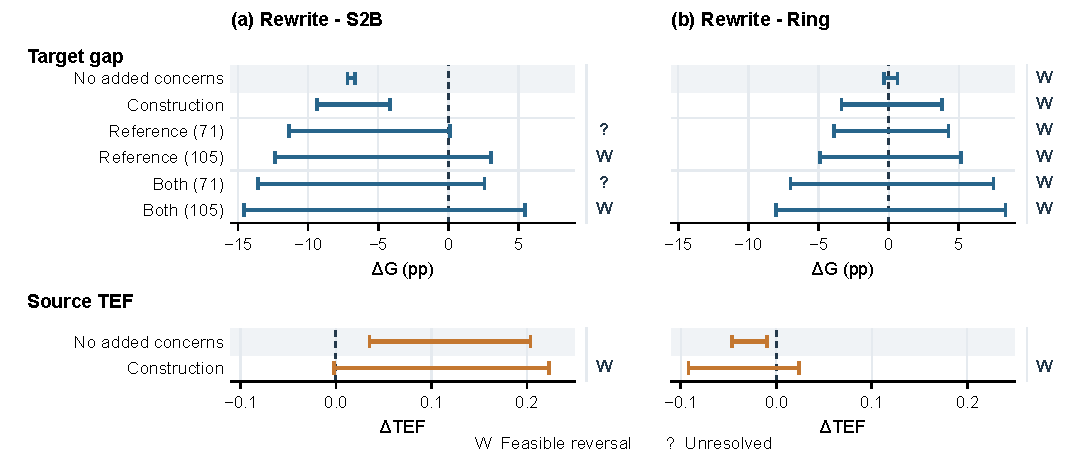
\includegraphics[width=\textwidth]{figures/current/Fig5.pdf}
\caption{Sensitivity of rewriting with fixed SQL using earlier audit flags. Target gap is above source TEF. W: a feasible score assignment reverses the comparison; ?: search unresolved; blank: not searched.}
\label{fig:risk-sources}
\end{figure*}

Construction flags preserve the rewrite's gap advantage but leave both TEF contrasts unresolved. Either reference-risk set makes gap direction unresolved without changing TEF.

Positive differences are feasible in 14/16 Verified cases whose bounds cross zero; this establishes neither semantic errors nor reversal probabilities.

Terra reviews 160 paired originals under the same protocol (Table~\ref{tab:audit-expanded}(c)). Combined flags cover 24 original, 43 rewritten, 23 Ring and 71 reference items. Verified rewrite-minus-original gap $[-0.142130,+0.032135]$ and TEF $[-0.008539,+0.235566]$ are both unresolved.

\subsubsection{Metric Weights and Model Coverage}\label{sec:sensitivity}
Accuracy and the correct-count CDF favor S2B against all comparators; disagreement favors it over Template, is adverse to Ring ($[+0.012123,+0.066481]$), and unresolved for Omni/Synth. Equal component weights and pooled-task averaging leave S2B-minus-Synth unresolved: $[-0.400081,+0.034253]$ and $[-0.430144,+0.025669]$. Template/Ring/Omni directions persist.

Figure~\ref{fig:weights} varies nonnegative accuracy/CDF/disagreement weights summing to 2.5 on the first Verified release without semantic flags. Colors classify regions as favorable, adverse or unresolved using conservative bounds, without assigning probabilities.

\begin{figure*}[t]
\centering
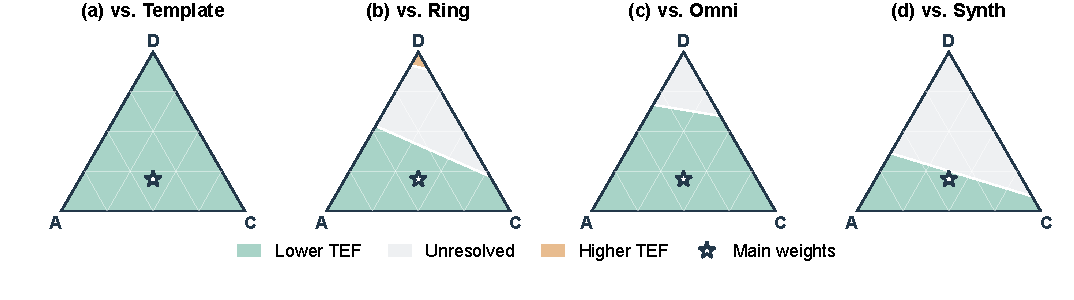
\includegraphics[width=\textwidth]{figures/current/Fig6.pdf}
\caption{Post-hoc TEF weight sensitivity. A: accuracy; C: correct-count CDF; D: disagreement. Star: original weights $(1,1,0.5)$.}
\label{fig:weights}
\end{figure*}

S2B beats Template throughout the weight region. Emphasizing disagreement can favor Ring and leaves Omni/Synth unresolved.

Removing Qwen retains favorable Verified TEF contrasts after recomputing normalizers; external adaptations still have lower gap (Table~\ref{tab:panel-coverage}). Summary/DDL source prompts both favor S2B over Template, with unresolved direct difference.

Broader coverage retains the Template--S2B gap advantage (Table~\ref{tab:panel-coverage}). Adding Qwen3.6-27B, Qwen3.8-27B, Gemma 3 4B and OLMo 2 7B tests model coverage, without resolving exclusion bias, transfer or training overlap.

\begin{table*}[t]\centering\small
\caption{Eight-database gap sensitivity: positive $I_G=G(\mathrm{Template})-G(\mathrm{S2B})$ favors S2B. Conditional confidence intervals (CIs) resample within domains; bounds describe unknown scores.}
\label{tab:panel-coverage}
\begin{tabular}{lrrrl}\toprule
Setting & Pairs & References & Gap improvement $I_G$ & Interpretation\\\midrule
Non-Qwen panel &2,000&906&$0.026560$&Ten-release mean\\
Broader reference coverage &3,778&982&$0.053302\ [0.041870,0.063207]$&Conditional 95\% CI\\
Equal-skeleton weighting &3,778&982&$0.046936\ [0.034298,0.057670]$&Conditional 95\% CI\\
Full available pool &3,835&1,118&$[0.009303,0.090704]$&Unknown-score bound\\\midrule
Fourteen models: strict &2,000&906&$[0.002662,0.059226]$&Unknown-score bound\\
Fourteen models: database checks &2,000&906&$[0.025795,0.032495]$&Unknown-score bound\\
Fourteen models: strict &3,778&906&$[0.002188,0.059640]$&Unknown-score bound\\
Fourteen models: database checks &3,778&906&$[0.025787,0.032648]$&Unknown-score bound\\\bottomrule
\end{tabular}

\smallskip\parbox{\textwidth}{\footnotesize The full-pool setting uses 8,788 prompts/model. The 2,000-pair fourteen-model rows average bound endpoints over ten overlapping releases. Fourteen-model concordances/inversions are 567/136 for 2,000 pairs and 533/168 for 3,778 pairs, each out of 728 dependent model pairs.}
\end{table*}

LIMIT counts are 1,739/2,000 for Template/S2B, 1,753 Ring, 424 Omni and 872 Synth, versus 62/906 references. Only 108/240 method--domain--structure cells (10/40 LIMIT cells) have ten tasks in both populations, preventing complete matched analysis. A pilot table-name repair does not apply to the retained failed outputs.

\subsection{Generalization Experiments}\label{sec:external}
\begin{table*}[t]\centering\small
\caption{External-pilot differences (S2B minus comparator); negative favors S2B. TACO: 750 tasks/method, 595 references, database and reference checks. BEAVER: 472 tasks/method, all 194 references. Scoring layers and schemas are separated. Each pilot uses matching source context, pooled TEF and gap averaged across domains.}
\label{tab:external-pilot}
\begin{tabular}{llrr}\toprule
Setting & Comparator & $\Delta\mathrm{TEF}$ & $\Delta G$\\\midrule
TACO: retrieved schema & Template & $[-0.006024,+0.016398]$ & $[-0.030517,+0.044555]$\\
TACO: retrieved schema & Ring & $[+0.133673,+0.280760]$ & $[+0.148866,+0.277121]$\\\midrule
BEAVER: retrieved, Base & Template & $[-0.146373,-0.033660]$ & $[-0.081035,+0.060364]$\\
BEAVER: retrieved, Base & Ring & $[-0.242054,-0.013075]$ & $[-0.056789,+0.099330]$\\
BEAVER: oracle schema, Base & Template & $[-0.142702,-0.028519]$ & $[-0.083884,+0.049262]$\\
BEAVER: oracle schema, Base & Ring & $[-0.130602,+0.168975]$ & $[-0.051570,+0.064633]$\\\midrule
BEAVER: retrieved, Verified & Template & $[-0.146163,-0.037765]$ & $[-0.081035,+0.060364]$\\
BEAVER: retrieved, Verified & Ring & $[-0.235815,-0.016203]$ & $[-0.056789,+0.099330]$\\\bottomrule
\end{tabular}\end{table*}

TACO OpenData \citep{deng2026taco} supplies two related Beijing databases and Connecticut, with potentially synthetic references. Admission and initial sampling differ from the main study. With 16 retrieved objects, contrasts are unresolved against Template and adverse against Ring (Table~\ref{tab:external-pilot}). Incomplete schemas limit semantic assessment; Omni/Synth miss 250-task quotas with incomplete runs.

A ten-model pilot uses CORE-T's SQLite-converted BEAVER \citep{chen2024beaver}.\footnote{\url{https://github.com/UKPLab/emnlp2026-core-t}} DW/Nova/Neutron supply unequal capacities of 250/198/24 tasks/method and all 121/43/30 references; Nova/Neutron share provenance. Retrieval covers required objects for 33/194 references. Oracle schemas use reference-SQL-selected tables/views and compact source DDL, hiding SQL. This tests known relevant schemas, changing coverage and input length; it does not test retrieval.

In both Base conditions, Schema2Bench's pooled TEF advantage over Template persists; against Ring it crosses zero with oracle schemas. Neutron's oracle TEF/gap favor Ring. Reference unknowns remain 660/1,940 and 663/1,940. Unresolved gap and wide rank/regret bounds do not establish better target model selection.

\paragraph{Seven-database diagnostic}
A separate ten-model diagnostic on the seven earlier databases finds no general Schema2Bench advantage. Equal-domain means of Verified direct TEF bounds are $[-0.1055,+0.0750]$, $[+0.0206,+0.2190]$, $[-0.5911,+0.1033]$ and $[-0.4155,+0.4507]$ for S2B minus Template, Ring, Omni and Synth fallback. These average domain contrasts, not pooled tasks. S2B beats Ring on TPC-H, loses on Chinook, Instacart, SFDFFD and TPC-DS, and is unresolved on IMDb/USAccidents.

Task counts vary: TPC-DS Omni uses 8,192 tokens; TPC-H Omni retains partial outputs; Synth uses fallback generation. Original qualification results remain unchanged. Independent target references are unverified, precluding gap, rank and regret claims.


\subsection{Discussion}\label{sec:discussion}

Schema2Bench is supported for source-preserving migration: it improves both objectives over Template and Verified TEF over the three external adaptations. Ring's lower gap and mean regret favor it for target model selection, despite fewer Astra-supported pairs (Table~\ref{tab:audit-expanded}). The preferred method therefore depends on the measurement objective.

Retrospective tolerance choices do not establish non-inferiority, which requires prospective margins and sufficient precision.

Most improvement precedes selection, whose contribution is bounded adjustment and coverage diagnosis. Screening, budgets and shared data restrict generalization. External results are mixed; semantic-risk bounds fix unflagged scores.

Table~\ref{tab:cost} includes failed-call tokens. Artifacts support offline score, feasibility and execution-evidence checks. Full reproduction needs external models, data and environments; redistribution rights remain unverified.


\section{Related Work}\label{sec:related}
\subsection{Text-to-SQL}
Text-to-SQL research improves schema linking, representation learning and constrained decoding \citep{wang2020ratsql,lin2020bridge,lei2020schemalinking,li2023resdsql,scholak2021picard}. DAIL-SQL studies prompting and example selection; CodeS develops specialized open models \citep{gao2024dailsql,li2024codes}. PURPLE retrieves demonstrations by operator composition; KaSLA models schema linking as knapsack optimization \citep{ren2024purple,yuan2026kasla}. Long-context NL2SQL studies how schema, values and context affect accuracy and latency \citep{chung2025longcontext}. These methods improve predictors; Schema2Bench constructs workloads to compare them on new databases.

DIN-SQL, MAC-SQL and SHARE use decomposition, collaboration or correction \citep{pourreza2023dinsql,wang2025macsql,qu2025share}; CycleSQL uses database-grounded explanations as feedback \citep{fan2025cyclesql}. These checks improve predictions but do not establish benchmark fidelity. Execution agreement itself requires qualification through test suites, formal checks and reference audits \citep{zhong2020testsuite,klopfenstein2026spotit,pourreza2023evaluating,liu2025nl2sqlbugs}.

Spider, BIRD and conversational benchmarks provide shared evaluation tasks \citep{yu2018spider,li2023bird,yu2019sparc,yu2019cosql}. Spider 2.0, KaggleDBQA, ScienceBenchmark, BEAVER and customer-log evaluations extend the range of database demands \citep{lei2025spider2,lee2021kaggledbqa,zhang2024sciencebenchmark,chen2024beaver,ganti2024failures}. Perturbation benchmarks isolate linguistic, knowledge, schema and query changes \citep{gan2021spidersyn,gan2021spiderdk,pi2022adveta,chang2023drspider,zhou2026sqlstructeval,perlitz2026polysql}. SQLMorph adds join expansion and fine-grained execution metrics; VLD-Bench studies discrepancies between question values and database entries \citep{malekpour2026sqlmorph,koukouvinis2026value}.

These diagnostics isolate failures under task changes, without establishing source fidelity or target alignment after migration. Following evidence-centered design and concurrence research \citep{liu2024ecbd,sun2023concurrence,kovatchev2024benchmark}, we separately assess source response profiles and target accuracy gaps, rankings and regret, retaining uncertainty when execution or semantic evidence is insufficient.

\subsection{Data Synthesis}
Synthetic question--SQL pairs support pretraining and adaptation \citep{yu2021grappa,li2021semiautomatic,lent2021canonical}. RingSQL instantiates schema-independent templates; OmniSQL synthesizes large-scale training data \citep{sterbentz2026ringsql,li2025omnisql}. SING-SQL, EvolSQL and SynSQL study other synthesis settings \citep{caferoglu2025singsql,pan2026evolsql,habibollah2026synsql}. These training objectives do not establish evaluation fidelity. We compare local adaptations at fixed workload sizes and isolate wording effects with SQL fixed.

Dataset distillation approximates learning from larger datasets with small synthetic training sets \citep{wang2018distillation,zhao2021condensation}; gradient-matching condensation matches training gradients. Schema2Bench instead constructs cross-database test workloads without updating evaluators. Distilled data are assessed through learned models; migrated benchmarks require validation of the model comparisons they support.

Data selection reduces training or evaluation cost \citep{xie2023dsir,albalak2024dataselection,perlitz2024efficient}. TinyBenchmarks estimates benchmark performance from selected items; SMART filters items; SubLIME and FAFI study rank preservation \citep{maiapolo2024tiny,gupta2025smart,saranathan2025sublime,gusev2026ranking}. Schema2Bench uses moment matching and benefit--cost exchanges \citep{bach2012herding,derezinski2019minimax,khuller1999budgeted} to control SQL composition under domain quotas. Migration also changes grounding and candidate populations. We bound fidelity changes from structural exchanges and diagnose shortages that selection cannot fix. Small additional selection gains and mixed external results delimit the benefits.

\FloatBarrier
\begin{samepage}
\section{Conclusion}
Schema2Bench combines Benchmark Construction, Workload Selection and Benchmark Evaluation for source-preserving migration. On eight BIRD databases, it improves both source fidelity and target gap over Template, and achieves lower TEF than three external adaptations under Verified scoring and declared weights. Most gain precedes selection; coverage bounds identify deficits selection cannot repair. Lower external target gaps, semantic uncertainty and mixed external-domain results delimit this advantage.

\label{closure:main-end}
\end{samepage}
